\documentclass[conf]{new-aiaa}
\usepackage[utf8]{inputenc}
\usepackage{graphicx}
\usepackage{amsmath}
\usepackage[version=4]{mhchem}
\usepackage{siunitx}
\usepackage{longtable,tabularx}
\setlength\LTleft{0pt} 
\usepackage{amsmath} %math symbols and equations
\usepackage{booktabs} %standard table support
\usepackage{graphicx} %include figures/images
\usepackage{float} %positioning of figures
\usepackage{multicol}  %able to use columns
\usepackage{tikz} %create graphics
\usepackage{pgfplots} %create graphics
\usepackage{lettrine} % make a fancy letter
\usepackage{subcaption}  %used to make subfigures

\newcommand\yesnumber{\addtocounter{equation}{1}\tag{\theequation}}



\title{Advancements in Aerodynamic Shape Optimization with Hybrid Laminar Flow Control for Infinite Swept and Finite Wings at Cruise Conditions}

\author{Justin M.\ Pascual \footnote{PhD Candidate, University of Toronto Institute for Aerospace Studies, AIAA Student Member, justin.pascual@mail.utoronto.ca} and David W.\ Zingg \footnote{Distinguished Professor of Computational Aerodynamics and Sustainable Aviation, University of Toronto Institute for Aerospace Studies, AIAA Associate Fellow, david.zingg@utoronto.ca}}
\affil{Institute for Aerospace Studies, University of Toronto, ON M3H 5T6}

\begin{document}

\maketitle

\begin{abstract}

Hybrid Laminar Flow Control (HLFC) offers a promising approach to reduce drag by extending laminar flow regions on wings through the combination of passive shaping and active boundary-layer suction. In this work, a suction boundary condition is integrated into a Reynolds-Averaged Navier–Stokes (RANS) aerodynamic shape optimization framework coupled with the SA-sLM2015cc local correlation-based transition model. The implementation is first validated against benchmark cases, including flat-plate flow and NACA 64A010 airfoil experiments, demonstrating accurate prediction of laminar-to-turbulent transition under varying suction intensities. Lift-constrained drag minimization is then performed for infinite swept wings under Airbus A340 and A350 operating conditions. Applying suction upstream of the transition location on optimized geometries further delays crossflow-dominated transition, yielding drag reductions of up to 20\% relative to baseline geometries and exceeding reductions achieved by natural laminar flow optimization alone. The study also examines the effects of suction extent, surface porosity, and suction drag and pump-power penalties, highlighting the trade-offs between performance gains and energy requirements. Future work will extend the framework to three-dimensional finite wings and incorporate optimization of suction power and placement to maximize aerodynamic efficiency while minimizing energy consumption, enabling realistic assessments of HLFC for practical aircraft designs.

\end{abstract}

\section{Nomenclature}

{\renewcommand\arraystretch{1.0}
\noindent\begin{longtable*}{@{}l @{\quad=\quad} l@{}}
$A$ & airfoil area \\
$b$ & span \\
$c$ & chord \\
$C_D$ & coefficient of drag \\
$C_L$ & coefficient of lift \\
$C_Q$ & coefficient of suction \\
$e$ & total energy per unit volume \\
$j$ & mass flux \\
$l$ & length of suction zone for a flat plate \\
$\dot{m}$ & mass flow rate per unit area \\
$M$ & Mach number \\
$Q_{\text{suc}}$ & total volumetric flow rate through the surface \\
$\mathbf{Q_{\text{target}}}$ & solution vector of the conservative flow variables at an individual node \\
$Re$ & Reynolds number \\
$v_{\text{suc}}$ & suction speed \\
$v_{\text{w}}$ & normal component of velocity \\
$U_\infty$ & free-stream velocity \\
$\Lambda$ & sweep angle \\
$\mu_\infty$ & free-stream dynamic viscosity \\
$\rho$ & density \\
$\rho_w$ & local density at the wall \\
$\rho_\infty$ & free-stream density \\
$\xi$ & curvilinear coordinate \\
\end{longtable*}}

\section{Introduction} \label{sec:introduction}

\lettrine[findent=2pt]{\textbf{T}}he commercial aviation industry has experienced significant growth over the past few decades. Excluding the temporary decline in travel due to the COVID-19 pandemic, demand for safe and efficient air travel has increased by approximately 6\% annually. This growing demand has heightened environmental concerns, driving interest in the development of more efficient aircraft designs. Aerodynamic shape optimization supports this effort by iteratively simulating and refining designs to improve specific performance metrics, offering a more systematic and effective alternative to traditional manual design iteration methods.

For a typical commercial aircraft, viscous drag contributes roughly 50\% of the overall drag while operating at cruise conditions \cite{bushnell_overview_1992}. As flow passes over a surface, it transitions from laminar to turbulent, with turbulent flow having higher frictional forces and a thicker boundary layer, increasing the overall drag. To delay this transition from laminar to turbulent flow, flow control methods can be implemented to push the transition location further downstream, increasing the regions of laminar flow \cite{green_civil_2003}. There are two main mechanisms through which flow transitions, the first being Tollmien-Schlichting (TS) instabilities, which occur in two-dimensional boundary layers in the form of vortices aligned in the spanwise direction. These instabilities are highly receptive to disturbances in the flow, and are amplified as they are advected downstream, resulting in the transition to turbulence \cite{green_civil_2006}. The second mechanism is crossflow (CF) instabilities, which arise on swept wings and are characterized by an inflection point in the transverse velocity profile. This inflection point causes the flow to be unstable, resulting in streamwise vortices that transition the flow to turbulence.

To improve aerodynamic efficiency by delaying the transition from laminar to turbulent flow, one promising passive approach is natural laminar flow (NLF), which relies on careful wing shaping to extend the laminar region. However, NLF design is challenging due to competing requirements for suppressing different instability modes. For example, favorable pressure gradients help delay Tollmien–Schlichting (TS) instabilities but tend to amplify crossflow (CF) instabilities. Similarly, increasing wing sweep reduces wave drag but intensifies CF instabilities, resulting in higher viscous drag. These conflicting effects of pressure gradients and sweep limitations mean that NLF is generally restricted to modest sweep angles and Reynolds numbers \cite{lynde_computational_2017,lynde_preliminary_2019}.

At higher sweep angles and Reynolds numbers, active laminar flow control becomes necessary. Hybrid Laminar Flow Control (HLFC) combines the passive shaping of NLF with active boundary-layer suction to delay transition further. By modifying the boundary-layer profile through shaping and suction, HLFC effectively postpones the onset of turbulence. The technique is particularly suited to wings and empennage due to their large wetted areas and typically high sweep, while nacelles and other components may rely on other drag-reduction strategies \cite{johansen_prediction_1999}.

The concept of applying suction across the full upper and lower surfaces of a wing was first experimentally explored by NACA in the Langley low-turbulence pressure tunnel \cite{Braslow1951}. Using a NACA 64A010 airfoil with a sintered bronze perforated surface, the study demonstrated that boundary-layer suction could maintain laminar flow at low speeds ($M \approx 0.3$) and moderate Reynolds numbers ($Re = 6 \times 10^6$).

NASA later extended these investigations in the Langley Laminar-Flow-Control Experiment \cite{bobbitt_results_1992, harvey_design_1986, dagenhart_design_1978, berry_boundary-layer_1987}, applying suction over both upper and lower wing surfaces of a supercritical airfoil in unswept and swept configurations. The study validated transition prediction methods and compared slotted and perforated suction surfaces, accounting for temperature gradients and surface porosity in the efficiency calculations. Results showed that suction could successfully delay transition up to 60\% of the chord, confirming the effectiveness of both surface types in moving the transition location downstream.

Building on these experimental studies, Fisher and Fischer demonstrated active laminar flow control on a JetStar aircraft during the Leading-Edge Flight Test (LEFT) \cite{fisher_development_1987}. The aircraft employed both slotted and perforated suction surfaces, with additional measures such as Krueger flaps with integrated deicer nozzles to protect against insect, ice, and particulate contamination. Both suction configurations were successfully implemented, with slotted surfaces proving more effective at delaying transition, while perforated surfaces were more prone to clogging.

On the computational side, Sudhi et al.\ applied active laminar flow control to two-dimensional airfoils using XFOIL coupled with an $e^N$ transition prediction method \cite{Sudhi2023-yf}. Drag-minimization optimizations were performed with and without suction, treating the onset of suction as a design variable. Optimized suction distributions applied upstream of the natural transition location delayed transition to 80\% of the chord and reduced drag by 30\% relative to the no-suction case. Extending this methodology, Sudhi et al.\ explored HLFC on transonic, infinite swept wings at high Reynolds numbers \cite{Sudhi2023-yf}. By jointly optimizing wing shape and suction distribution using a multi-objective genetic algorithm, HLFC configurations achieved up to 25\% drag reduction over NLF designs at $Re = 30 \times 10^6$ and sweep angle $22.5^\circ$, outperforming fully turbulent designs by 27\%. Prasannakumar et al.\ \cite{Prasannakumar_Sudhi_Seitz_Badrya_2024} applied suction to a finite wing swept at $16^\circ$ at the operating conditions of a hybrid-electric propulsion aircraft. The aircraft has a cruise Mach number of 0.71, $C_L = 0.5$ and a range of 4600 km. The objective of this work was to maximize the laminar region while minimizing the suction and pressure drag through the control of suction panels at different spanwise stations at the leading edge. The results of this study indicate that the transition point is able to be moved to 60\% chord with considerations for a battery powering the suction system to maximize the net drag reduction.

Pascual and Zingg \cite{Pascual2025-bx} implemented a suction-based aerodynamic optimization framework for HLFC, coupling a suction boundary condition with the SA-sLM2015cc transition model \cite{piotrowski_compressibility_2023} in a RANS solver. Strategically placing multiple suction locations yielded significant drag reductions. On an RAE2822 airfoil, suction applied upstream of the transition location reduced drag by 6\% at a suction speed of $0.1\% \: U_\infty$. For infinite swept wings, aerodynamic shaping alone achieved 5\% drag reduction, while applying suction upstream resulted in 8\% drag reduction, validating the flow physics and demonstrating that these operating conditions are achievable within the limits of NLF.

The objective of the current work is to develop an effective methodology to perform aerodynamic shape optimization in the presence of laminar-turbulent transition and suction, and to use the optimization methodology developed to study optimal approaches to drag reduction via HLFC and to quantify the performance benefits achievable. To validate the suction boundary condition implementation, several benchmark cases are examined, including flat-plate flow, airfoil experiments, and high-speed swept-wing configurations.

Section \ref{sec:methodology} outlines the flow solver, transition-prediction model, and aerodynamic shape optimization framework, including the modeling of active laminar flow control. Section \ref{sec:validation} presents the validation cases performed on flat plates and airfoils. Section \ref{sec:results} presents the results of lift-constrained drag minimization of two-dimensional airfoils with and without sweep and finite wings, incorporating suction in various ways. Finally, conclusions and future work are presented in Section \ref{sec:conclusion}.

\section{Methodology} \label{sec:methodology}

Aerodynamic shape optimization is carried out using Jetstream, the high-fidelity optimization framework developed at the University of Toronto Institute for Aerospace Studies. Jetstream comprises five core components: a Newton-Krylov-Schur flow solver for the Reynolds-Averaged Navier–Stokes (RANS) equations \cite{osusky_parallel_2008, osusky_parallel_2010}; a transition-prediction model based on empirical local correlations, coupled with the one-equation Spalart–Allmaras (SA) turbulence model \cite{piotrowski_investigation_2019, piotrowski_smooth_2021}; a unified geometry parameterization and mesh deformation scheme based on linear elasticity \cite{hicken_aerodynamic_2010}; the SNOPT gradient-based optimizer used alongside a discrete-adjoint gradient method \cite{gill_snopt_2002}; and a combination of free-form deformation (FFD) and axial deformation for geometry control \cite{gagnon_two-level_2015}. The framework has been extended to support active boundary-layer suction through the implementation of a suction boundary condition.

\subsection{RANS Flow Solver} \label{sec:diablo}
The flow solver, Diablo \cite{osusky_parallel_2008, osusky_parallel_2010}, is a multiblock, parallel, implicit solver that employs second-order summation-by-parts (SBP) operators for spatial discretization and uses simultaneous approximation terms (SATs) \cite{delrey_fernandez_simultaneous_2018} to enforce boundary and block interface conditions. SATs act as penalty terms that drive the solution toward a specified target state at the boundaries. The SBP-SAT discretization of the governing equations results in a nonlinear system, which is solved using Newton’s method in two distinct phases: an approximate-Newton phase followed by an inexact-Newton phase. In the first phase, an approximate Jacobian is used in conjunction with the implicit Euler method, with a gradual increase in time step. In the second phase, matrix-free matrix-vector products are used to approximate the exact Jacobian, enabling a more aggressive time step ramp-up. The transition between phases is triggered when the total residual decreases by five orders of magnitude. In both phases, the resulting linear systems are solved using the preconditioned Krylov iterative solver GMRES.

\subsection{Transition Prediction Model} \label{sec:transition-prediction}
The flow solver incorporates boundary-layer transition prediction using the SA-sLM2015cc model developed by Piotrowski and Zingg \cite{piotrowski_investigation_2019, piotrowski_smooth_2021, piotrowski_investigation_2022}. This model builds on the $\gamma\text{-}Re_{\theta t}$ framework; an empirical, correlation-based approach introduced by Langtry and Menter \cite{langtry_correlation-based_2009} to model Tollmien–Schlichting (TS) and crossflow (CF) instabilities. The $\gamma\text{-}Re_{\theta t}$ model includes two transport equations: one for $\gamma$, the intermittency function, and another for $Re_{\theta t}$, the momentum-thickness Reynolds number. The SA-sLM2015 model couples this transition framework with the one-equation Spalart–Allmaras turbulence model \cite{spalart_one-equation_1994}, and replaces non-smooth functions in the original formulation with smoothed alternatives to ensure a continuous and differentiable design space. Piotrowski and Zingg later enhanced the model by incorporating compressibility corrections for both TS and CF instabilities, leading to the current version, SA-sLM2015cc \cite{piotrowski_compressibility_2023}.

\subsection{Geometry Parametrization, Mesh Deformation, Geometry Control} \label{sec:mesh-movement}

The optimization framework integrates geometry parameterization with mesh deformation, following the method developed by Hicken and Zingg \cite{hicken_aerodynamic_2010}. Each computational grid block is linked to a B-spline volume, where the control points on the surface provide a low-dimensional representation of the original geometry. A mesh deformation technique based on linear elasticity transmits changes in the surface control points to the interior mesh through the control volume. Geometry manipulation is handled using a hybrid approach that combines free-form and axial deformation methods \cite{gagnon_two-level_2015}. The free-form deformation (FFD) volumes are constructed using B-spline volumes, while the axial curves are represented by B-spline curves. The FFD control points govern section shape, chord, and twist, whereas the axial control curves manage sweep, span, and dihedral. The deformation of the axial control curves is not needed for the infinite swept wing cases considered in this paper, but is used for the finite wing optimization cases.

\subsection{Gradient-Based Optimization} \label{sec:snopt}

The optimization process is performed using SNOPT \cite{gill_snopt_2002}, a gradient-based algorithm that operates within a sequential quadratic programming (SQP) framework and is capable of handling both linear and nonlinear constraints. Gradient information is obtained through the discrete-adjoint method \cite{Jameson1998-sf, Osusky2015-qh}.

\subsection{Suction Boundary Condition} \label{sec:suction-bc}

To simulate suction on the wing surface, the boundary is treated as a no-slip wall with a prescribed normal velocity directed into the surface. This is implemented by modifying the simultaneous approximation term (SAT) associated with the no-slip adiabatic wall condition. In particular, the momentum terms at the boundary are adjusted to account for the imposed suction velocity. The solution vector, $\textbf{Q}_\text{target}$, modified for the suction boundary condition is defined as:
\begin{equation}
	\textbf{Q}_{\text{target}} = \begin{bmatrix}
	\vspace{0.3 cm}
	\rho \\ \vspace{0.3 cm}
	\displaystyle \frac{\frac{\partial \xi}{\partial x} \cdot v_{\text{suc}} \cdot \rho}{\sqrt{\left(\frac{\partial \xi}{\partial x}\right)^2+\left(\frac{\partial \xi}{\partial y}\right)^2 + \left(\frac{\partial \xi}{\partial z}\right)^2}} \\ \vspace{0.3 cm}
	\displaystyle \frac{\frac{\partial \xi}{\partial y} \cdot v_{\text{suc}} \cdot \rho}{\sqrt{\left(\frac{\partial \xi}{\partial x}\right)^2+\left(\frac{\partial \xi}{\partial y}\right)^2 + \left(\frac{\partial \xi}{\partial z}\right)^2}} \\ \vspace{0.3 cm}
	\displaystyle \frac{\frac{\partial \xi}{\partial z} \cdot v_{\text{suc}} \cdot \rho}{\sqrt{\left(\frac{\partial \xi}{\partial x}\right)^2+\left(\frac{\partial \xi}{\partial y}\right)^2 + \left(\frac{\partial \xi}{\partial z}\right)^2}} \\ \vspace{0.3 cm}
	e
	\end{bmatrix},
	\label{eq:Qwall}
\end{equation}
\noindent where $v_{\text{suc}} < 0$ is the user-defined suction speed parameter and $\xi$ is the curvilinear coordinate direction normal to the surface. The implementation of Equation \ref{eq:Qwall} with the appropriate inviscid and viscious SATs to create a suction boundary condition is described in \cite{Pascual2025-bx}. Suction is implemented using a specified suction speed, $v_{\text{suc}}$, as stated above, and is analyzed and plotted across the surface using the suction coefficient, $C_Q$, which is defined as:
\begin{equation}
C_Q = \frac{\rho_w v_{\text{suc}}}{\rho_\infty U_\infty}
\label{eq:Cq}
\end{equation}

\noindent where $\rho_w$ and $\rho_\infty$ represent the local wall density and the free-stream velocity, respectively. 

\subsubsection{Suction Drag Considerations}

The suction boundary condition formulation accounts for the drag effects introduced by active boundary-layer control. The suction drag represents the additional skin-friction component arising from the extraction of low-momentum fluid near the surface, which alters the boundary-layer velocity profile and increases the local wall shear stress. Following Fehrs \cite{Fehrs2020-qg}, the suction drag coefficient over a unit surface is expressed as:
\begin{equation}
\begin{aligned}
C_{D,\text{suc}} &= \frac{2 \cdot D_{\text{suc}}}{\rho_\infty U_\infty^2 	bl} = -2 \cdot \frac{v_w}{U_\infty}  = 2 \cdot C_Q.
\label{eq:suction-drag}
\end{aligned}
\end{equation}

\noindent This formulation relates the prescribed suction velocity to the additional skin-friction drag.

\subsubsection{Suction Pump Power Considerations}

Additionally, active suction requires energy to sustain the prescribed mass flux through the porous surface, which can be expressed as an equivalent power drag coefficient. Following the formulation of Prasannakumar et al.\ \cite{prasannakumar_design_2022} and assuming the pump efficiency, $\eta_p = 1$, the ideal suction pump power penalty is given by:

\begin{equation}
C_{D,\text{pump}} = \left( \frac{U_e}{U_\infty} \right)^2 \left( \frac{v_{\text{suc}}}{U_\infty} \right).
\label{eq:suction-pump-power}
\end{equation}

\noindent This expression captures the energy cost of suction in a compact form, allowing it to be directly incorporated into aerodynamic optimization as an equivalent drag contribution.

\section{Model Validation}
\label{sec:validation}
This section presents the validation of the developed suction boundary condition. First, three validation cases are discussed: boundary-layer suction applied to a flat plate and to a NACA 64A010 airfoil, demonstrating agreement with both computational and experimental reference data. The third case uses a NASA LFC supercritical infinite swept wing operated at HLFC-capable conditions and will be included in the full paper. 

\subsection{Boundary-layer Suction Applied to a Flat Plate}
Fehrs implemented a no-slip wall boundary condition using an effusion mass flux boundary condition in the DLR TAU-Code \cite{Fehrs2020-qg} and validated it analytically. 	The operating conditions consist of $U_\infty = 40$ m/s, $Re = 6.62 \times 10^6$ with the suction coefficient and suction velocity listed in Table \ref{tab:Fehrs_operating_conditions}. The results in Figure \ref{fig:fehrs_flat_plate} show the velocity profiles with respect to the similarity variable $\eta$, which is defined as:
\[
\eta = y \sqrt{\frac{U_\infty}{2 \nu x}}.
\]
The present computational results show excellent agreement with the reference data, with the algebraic transition model results to be shown in the full paper.

\addtocounter{table}{-1}
\begin{table}[!t]
\centering
\caption{Inflow conditions for flat plate with boundary-layer suction}
\label{tab:Fehrs_operating_conditions}
\begin{tabular}{ccccc}
\toprule
Case & $C_Q$ & $v_w$ (m/s)\\
\midrule 
1 & $8.33 \times 10^{-4}$ & - 0.03342 \\
2 & $4.16 \times 10^{-3}$ & - 0.16712 \\
\bottomrule
\end{tabular}
\end{table}

\begin{figure}[!t]
\centering
\includegraphics[height = 8cm, width = \textwidth, keepaspectratio]{fehrs_flat_plate.pdf}
\caption{Boundary-layer velocity profiles with two different suction coefficients produced using the SA-sLM2015cc transition model validated against DLR TAU-Code computational results (shown with symbols).}
\label{fig:fehrs_flat_plate}
\end{figure}

\pagebreak

\subsection{Flow over an Airfoil with Prescribed Suction} \label{sub:workshop-infinite-swept}
Braslow et al.\ conducted experiments using a NACA 64A010 airfoil with a sintered bronze surface through which suction was applied \cite{Braslow1951}. Suction was applied across the entirety of the upper and lower surfaces, aside from a small portion at the leading edge at approximately $5\% \: x/c$. The wind tunnel was operated at a speed of $M \approx 0.3$ and $Re = 6 \times 10^6$ and the airfoil was fixed at $\alpha = 0^\circ$. The computational mesh used for this validation case is a 270 $\times$ 182 O-grid.
	
The experiment measured the boundary-layer profiles at 83\% of the chord and found that the flow was able to remain laminar. The results of this validation case are shown in Figure \ref{fig:Braslow_results}, with the computational results showing a laminar boundary-layer profile in agreement with the experimental results. 

\begin{figure}[!t]
\centering
\includegraphics[height=8cm, width = \textwidth, keepaspectratio]{braslow.pdf}
\caption{Boundary-layer velocity profiles at $\mathbf{83\%}$ chord comparing results obtained with the SA-sLM2015cc transition model to the NACA 64A010 wind tunnel experiment.}
\label{fig:Braslow_results}
\end{figure}

\begin{figure}[!t]
\centering
\includegraphics[height=8cm, width = \textwidth, keepaspectratio]{schwartzberg_extents.pdf}
\caption{Extent of laminar flow on the upper surface with various suction coefficients}
\label{fig:Schwartzberg_results}
\end{figure}

\begin{figure}[!t]
\centering
\includegraphics[height=8cm, width = \textwidth, keepaspectratio]{bl_profiles.pdf}
\caption{Boundary-layer profiles comparing experimental results with the present work for various suction coefficients}
\label{fig:bl_profiles}
\end{figure}

With the same experimental operating conditions, geometry and suction application, Schwartzberg et al.\ captured boundary-layer profiles for several suction coefficients and analyzed the effect this variation had on the transition front \cite{Schwartzberg1952}. Fehrs also used the DLR-TAU code to replicate this experiment \cite{Fehrs2020-qg}. To compare against experimental data, the transition location for $C_Q=0$ must be matched, and to account for the surface roughness, Fehrs used a turbulence intensity of $Tu=0.6\%$. The cases run in the present work use a turbulence intensity of $Tu=0.63\%$. The results comparing the computational and experimental transition locations are plotted in Figure \ref{fig:Schwartzberg_results} with the present work demonstrating close agreement with both the experimental and the computational results. Boundary-layer profiles were captured as part of this experiment and are shown in Figure \ref{fig:bl_profiles}, comparing the experimental results with the present work. When a lower suction velocity of $C_Q = 0.00076$ is used, the profile has a thicker profile, which is more characteristic of a turbulent boundary-layer profile. When suction is increased to a velocity of $C_Q = 0.00310$, a thinner profile is obtained. These results show close agreement with the experimental values providing validation for the current methodology.

\section{Optimization Results} \label{sec:results}
The methodology is applied to aerodynamic optimization studies involving infinite swept wings, where suction is applied to optimized geometries through discrete slot implementations. This study aims to quantify the aerodynamic performance improvements achievable through the integration of active laminar flow control into the design process.

\subsection{Suction Applied to an Optimized Geometry at Airbus A340 Operating Conditions}
\label{sub:a340-infinite-swept}
The following cases were completed using the RAE2822 airfoil as the initial geometry. This geometry is operated at Airbus A340 conditions consisting of $M = 0.82$, $Re = 45.34 \times 10^6$, $C_L = 0.512$, $\Lambda = 30^\circ$. The computational meshes used for this infinite swept wing are 360 $\times$ 120 O-grids. This geometry has 11 axial free-form deformation curves for each surface. Suction is applied at a fixed location on a geometry obtained from a lift-constrained drag minimization without suction, subject to an area constraint and minimum thickness constraints. The optimization problem is summarized as:
\begin{align*}
	\min_{\textbf{X}} \quad \quad &C_D(\textbf{X}) \quad \quad \\
	\text{s.t.} \quad \quad
		&C_L =  0.512 \yesnumber \label{eq:a340_opt_problem} \\
		&A \geq A_{\text{init}} \\
		&t/c \geq 0.15 (t/c)_{\text{init}},
\end{align*}
\noindent where \textbf{X} represents the design variable vector, including the angle of attack and the FFD control points, $C_L$ and $C_D$ the lift and drag coefficients, respectively, $A$ the cross-sectional area, and $t/c$ the thickness-to-chord ratio for each FFD control point pair. The `init' subscript indicates the value of the quantity from the baseline geometry. Previous results by Pascual and Zingg \cite{Pascual2025-bx} investigated lower sweep angle and Reynolds number combinations. The present work shifts focus to conditions where aerodynamic shaping offers limited benefits, increasing reliance on active suction to delay transition and reduce drag. The presented cases account for a suction drag penalty defined in Equation \ref{eq:suction-drag}, with suction being applied over the entire leading edge up until the upper and lower surface's respective transition locations on the optimized geometry, as in Figure \ref{fig:rae2822-suction-schematic}.

\begin{figure}[!t]
\centering
\includegraphics[height = \textheight, width = 8cm, keepaspectratio]{rae2822-suction-schematic.png}
\caption{Schematic depicting the distribution of suction over the entire leading edge until 9\% on the upper surface and 3\% on the lower surface.}
\label{fig:rae2822-suction-schematic}
\end{figure}

The results for the application of suction to both the upper and lower surfaces upstream of the transition location are shown in Table \ref{tab:a340-results}. Figure \ref{fig:a340-cpcf} shows that the pressure and friction coefficient plots for the baseline, NLF-optimized, and suction configurations. As seen int eh table, the NLF optimization provides an 11.8\% reduction in drag, but the optimizer still struggles to substantially delay transition on both surfaces, especially on the lower surface. 

When active suction is introduced, further drag reduction is achieved. When active suction is introduced, the aerodynamic performance improves further. Even the lowest suction level tested ($C_Q = 0.0001$) reduces drag to 59.17 counts, resulting in a 16.4\% drag reduction relative to the baseline. Increasing the suction coefficient consistently enhances the delay of transition, with $C_Q = 0.0010$ producing the lowest drag of 56.55 counts, corresponding to a 20.1\% reduction. 

Figure \ref{fig:a340-transition-plot} illustrates the influence of suction on the transition location for both surfaces. As expected, higher suction velocities push the transition point further downstream. However, the spacing between transition locations decreases with increasing $C_Q$, indicating diminishing returns in transition delay at higher suction levels. Overall, while all suction levels produce substantial improvements relative to the NLF-optimized case, the marginal benefit decreases as the suction intensity is increased, suggesting that there is an optimal value for the suction coefficient.

\begin{table}[!t]
\centering
\caption{Summary of results for the Airbus A340 case with suction applied along the entire leading edge, extending to 9\% of the chord on the upper surface and 2.5\% on the lower surface.}
\label{tab:a340-results}
\begin{tabular}{cccc}
\toprule
Configuration & $C_D$ (counts) & $L/D$ \\
\midrule 
Baseline  & 70.77 &  72.35\\
Turbulent Optimized  & 62.40 (-6.11\%) &  77.05\\
NLF Optimized & 62.39 (-11.8\%) & 82.04 \\
\midrule
$C_Q = 0.0001$ & 59.17 (-16.4\%) & 87.69 \\
$C_Q = 0.0005$ & 57.29 (-19.0\%) & 92.18 \\
$C_Q = 0.0010$ & 56.55 (-20.1\%) & 94.36 \\
\bottomrule
\end{tabular}
\end{table}

\begin{figure}[!t]
\centering
\includegraphics[height = 10cm, width = \textwidth, keepaspectratio]{cpcf.pdf}
\caption{Pressure and friction coefficient plots at Airbus A340 operating conditions with suction applied along the entire leading edge, extending to 9\% of the chord on the upper surface and 2.5\% on the lower surface.}
\label{fig:a340-cpcf}
\end{figure}

\begin{figure}[!t]
\centering
\includegraphics[height = 10cm, width = \textwidth, keepaspectratio]{transition_plot.pdf}
\caption{Transition location on the upper and lower surface at Airbus A340 operating conditions for various suction velocities when applied to the optimized geometry.}
\label{fig:a340-transition-plot}
\end{figure}

\subsubsection{Application of Suction at the Updated Transition Location}
BLURB HERE!

\begin{table}[!t]
\centering
\caption{Summary of results for the Airbus A340 case with suction applied along the entire leading edge, extending to 9\% of the chord on the upper surface and 2.5\% on the lower surface.}
\label{tab:a340-results-2}
\begin{tabular}{cccc}
\toprule
Configuration & $C_D$ (counts) & $L/D$ \\
\midrule 
Baseline  & 70.77 &  72.35\\
Turbulent Optimized  & 62.40 (-6.11\%) &  77.05\\
NLF Optimized & 62.39 (-11.8\%) & 82.04 \\
\midrule
$C_Q = 0.0001$ & 59.17 (-16.4\%) & 87.69 \\
$C_Q = 0.0005$ & 57.29 (-19.0\%) & 92.18 \\
$C_Q = 0.0010$ & 56.55 (-20.1\%) & 94.36 \\
\bottomrule
\end{tabular}
\end{table}

\begin{figure}[!t]
\centering
\includegraphics[height = 10cm, width = \textwidth, keepaspectratio]{cpcf.pdf}
\caption{Pressure and friction coefficient plots at Airbus A340 operating conditions with suction applied along the entire leading edge, extending to 9\% of the chord on the upper surface and 2.5\% on the lower surface.}
\label{fig:a340-cpcf-2}
\end{figure}

\begin{figure}[!t]
\centering
\includegraphics[height = 10cm, width = \textwidth, keepaspectratio]{transition_plot.pdf}
\caption{Transition location on the upper and lower surface at Airbus A340 operating conditions for various suction velocities when applied to the optimized geometry.}
\label{fig:a340-transition-plot-2}
\end{figure}

\subsection{Suction Applied to an Optimized Geometry at Airbus A350 Operating Conditions}

This geometry is operated at Airbus A350 conditions consisting of $M = 0.85$, $Re = 38.01 \times 10^6$, $C_L = 0.478$, $\Lambda = 31.9^\circ$. The computational meshes used for this infinite swept wing are 360 $\times$ 120 O-grids. This geometry has 11 axial free-form deformation curves for each surface.

The results for the application of suction to both the upper and lower surfaces upstream of the transition location are shown in Table \ref{tab:a350-results}, with suction applied along the entire leading edge, extending to 9\% of the chord on the upper surface and 2\% on the lower surface. The NLF-optimized shape provides a large improvement, reducing the drag to 55.09 counts (40.58\% drag reduction). When active suction is introduced, additional drag reduction is achieved beyond that obtained through shaping alone. The lowest suction coefficient tested ($C_Q = 0.0001$) decreases the drag to 52.68 counts, corresponding to a 43.18\% reduction relative to the baseline. As the suction level is increased, the drag continues to decrease, reaching 50.56 counts for $C_Q = 0.0010$, although the marginal improvement diminishes between the two highest suction levels. Similar to the cases previously shown, the results demonstrate that the A350 configuration benefits significantly from both aerodynamic shaping and active suction, with the combined approach providing the largest improvements with diminishing returns at higher suction intensities.

\begin{table}[!t]
\centering
\caption{Summary of results for the Airbus A350 case with suction applied along the entire leading edge, extending to 9\% of the chord on the upper surface and 2\% on the lower surface.}
\label{tab:a350-results}
\begin{tabular}{cccc}
\toprule
Configuration & $C_D$ (counts) & $L/D$ \\
\midrule 
Baseline  & 92.72 & 51.55 \\
Turbulent Optimized  & 62.40 (-32.70\%) & 76.63 \\
NLF Optimized & 55.09 (-40.58\%) & 88.51 \\
\midrule
$C_Q = 0.0001$ & 52.68 (-43.18\%) & 91.85 \\
$C_Q = 0.0005$ & 50.89 (-45.11\%) & 96.39\\
$C_Q = 0.0010$ & 50.56 (-45.47\%) & 97.43 \\
\bottomrule
\end{tabular}
\end{table}

\begin{figure}[!t]
\centering
\includegraphics[height = 10cm, width = \textwidth, keepaspectratio]{cpcf.pdf}
\caption{Pressure and friction coefficient plots at Airbus A350 operating conditions with suction applied along the entire leading edge, extending to 9\% of the chord on the upper surface and 2\% on the lower surface.}
\label{fig:a350-cpcf}
\end{figure}

\begin{figure}[!t]
\centering
\includegraphics[height = 10cm, width = \textwidth, keepaspectratio]{transition_plot.pdf}
\caption{Transition location on the upper and lower surface at Airbus A350 operating conditions for various suction velocities when applied to the optimized geometry.}
\label{fig:a350-transition-plot}
\end{figure}

\subsubsection{Application of Suction at the Updated Transition Location}
BLURB HERE!

\begin{table}[!t]
\centering
\caption{Summary of results for the Airbus A340 case with suction applied along the entire leading edge, extending to 9\% of the chord on the upper surface and 2.5\% on the lower surface.}
\label{tab:a350-results-2}
\begin{tabular}{cccc}
\toprule
Configuration & $C_D$ (counts) & $L/D$ \\
\midrule 
Baseline  & 70.77 &  72.35\\
Turbulent Optimized  & 62.40 (-6.11\%) &  77.05\\
NLF Optimized & 62.39 (-11.8\%) & 82.04 \\
\midrule
$C_Q = 0.0001$ & 59.17 (-16.4\%) & 87.69 \\
$C_Q = 0.0005$ & 57.29 (-19.0\%) & 92.18 \\
$C_Q = 0.0010$ & 56.55 (-20.1\%) & 94.36 \\
\bottomrule
\end{tabular}
\end{table}

\begin{figure}[!t]
\centering
\includegraphics[height = 10cm, width = \textwidth, keepaspectratio]{cpcf.pdf}
\caption{Pressure and friction coefficient plots at Airbus A340 operating conditions with suction applied along the entire leading edge, extending to 9\% of the chord on the upper surface and 2.5\% on the lower surface.}
\label{fig:a350-cpcf-2}
\end{figure}

\begin{figure}[!t]
\centering
\includegraphics[height = 10cm, width = \textwidth, keepaspectratio]{transition_plot.pdf}
\caption{Transition location on the upper and lower surface at Airbus A340 operating conditions for various suction velocities when applied to the optimized geometry.}
\label{fig:a350-transition-plot-2}
\end{figure}

%\subsection{Suction Applied to an Optimized Geometry at Boeing 747 Operating Conditions}
%
%This geometry is operated at Boeing 747 conditions consisting of $M = 0.854$, $Re = 55.14 \times 10^6$, $C_L = 0.457$, $\Lambda = 37.5^\circ$. The computational meshes used for this infinite swept wing are 360 $\times$ 120 O-grids. This geometry has 11 axial free-form deformation curves for each surface.
%
%The results for the application of suction to both the upper and lower surfaces upstream of the transition location are shown in Table \ref{tab:b747-results}. Figure \ref{fig:b747-cpcf} shows that the pressure and friction coefficient plots for the baseline and optimized geometry, and one with active suction (applied at $0.1\% \: U_\infty$) for clarity. For this preliminary optimization, the optimizer is struggling to delay transition on both surfaces. When active suction is applied, it can be seen that the upper surface's transition location is moved downstream for the case shown, resulting in a 10.6\% reduction in drag. The effect of $C_Q$ on the transition location is shown in Figure \ref{fig:b747-transition-plot}, which depicts both the upper and lower surfaces for the suction velocities used in this test. As expected, the transition location is pushed further downstream when a higher suction velocity is used, with substantial benefits compared to the preliminary NLF-optimized case shown with the blue markers.
%
%\begin{table}[!t]
%\centering
%\caption{Summary of results for infinite swept wing with suction. For the optimized geometry, the suction boundary condition is placed at 4\% of the chord with an extent of 1.5\% upstream.}
%\label{tab:b747-results}
%\begin{tabular}{cccc}
%\toprule
%Configuration & $C_D$ (counts) & $L/D$ \\
%\midrule 
%Baseline  & 73.88 & 68.22 \\
%NLF Optimized & 68.11 (-7.80\%) & 73.16 \\
%\midrule
%$C_Q = 0.0001$ & 67.46 (-8.69\%) & 74.23 \\
%$C_Q = 0.0005$ & 66.04 (-10.61\%) & 76.67\\
%$C_Q = 0.0010$ & 64.14 (-13.18\%) & 80.36 \\
%$C_Q = 0.0050$ & 64.14 (-13.18\%) & 80.36 \\
%
%\bottomrule
%\end{tabular}
%\end{table}
%
%\begin{figure}[!t]
%\centering
%\includegraphics[height = 10cm, width = \textwidth, keepaspectratio]{cpcf.pdf}
%\caption{Pressure and friction coefficient plots for cases involving the application of suction to both the upper and lower surface of an optimized geometry. Suction is applied at approximately 3\% of the wing chord on both surfaces.}
%\label{fig:b747-cpcf}
%\end{figure}
%
%\begin{figure}[!t]
%\centering
%\includegraphics[height = 10cm, width = \textwidth, keepaspectratio]{transition_plot.pdf}
%\caption{Transition location on the upper and lower surface for various suction velocities when applied to the optimized geometry.}
%\label{fig:b747-transition-plot}
%\end{figure}

\subsection{Suction Drag and Suction Pump Power Penalty Considerations}
This section evaluates the penalty implications associated with the suction drag, defined in Equation \ref{eq:suction-drag}, and suction-pump requirements, defined in Equation \ref{eq:suction-pump-power}, providing insight into their influence on the overall performance of the HLFC system. The following cases were completed with the same geometry and operating conditions as Section \ref{sub:a340-infinite-swept} for the Airbus A340. The results in Table \ref{tab:penalty-considerations} show the application of suction over the leading edge of the wing, as shown in Figure \ref{fig:rae2822-suction-schematic}, penalties for suction drag, suction pump power, and a combination of both considered, for various suction coefficients. The results demonstrate that for suction coefficients less than $C_Q = 0.0001$, the amount of drag from both suction drag penalties is nearly negligible, with the combination contributing 0.29\%. When suction power is increased, as shown with $C_Q = 0.0005$ and $0.0010$, the suction drag has an expected increasing contribution to the drag. When a relatively high suction coefficient of $C_Q=0.0050$ is used, the suction applied becomes excessive, no longer providing stabilization but rather increasing drag and potentially triggering earlier turbulent transition.

\begin{table}[!t]
\centering
\caption{Summary of results for infinite swept wing with suction at Airbus A340 operating conditions. Combinations of two different suction penalties are considered while varying the suction coefficient.}
\label{tab:penalty-considerations}
\begin{tabular}{cccc}
\toprule
Penalty & $C_D$ (counts) & $L/D$ \\
\midrule
$\mathbf{C_Q = 0.0001}$ & & \\
No Penalty  & 59.07 &  87.84 \\
Suction Drag & 59.17 (0.17\%) & 87.69 \\
Pump Power & 59.14 (0.12\%) & 87.74 \\
Combined & 59.24 (0.29\%) & 87.58 \\
\midrule
$\mathbf{C_Q = 0.0005}$ & & \\
No Penalty  & 56.79 & 93.01 \\
Suction Drag & 57.29 (0.88\%) & 92.18 \\
Pump Power & 57.13 (0.60\%) & 92.44 \\
Combined & 57.63 (1.48\%) & 91.62 \\
\midrule
$\mathbf{C_Q = 0.0010}$ & & \\
No Penalty  & 55.55 & 96.09 \\
Suction Drag & 56.55 (1.80\%) & 94.36 \\
Pump Power & 56.23 (1.22\%) & 94.89 \\
Combined & 57.24 (3.04\%) & 93.21 \\
\midrule
$\mathbf{C_Q = 0.0050}$ & & \\
No Penalty  & 59.29 & 87.53 \\
Suction Drag & 64.31 (8.47\%) & 80.63 \\
Pump Power & 62.68 (5.72\%) & 82.62 \\
Combined & 67.71 (14.20\%) & 76.35 \\
\bottomrule
\end{tabular}
\end{table}

\subsection{Suction Extent and Porosity Considerations}
This section investigates the influence of varying suction extent on the transition front, while maintaining a constant $C_Q$, and also incorporates local wall-shear effects by prescribing a node-wise porosity factor that reflects the shear conditions at each surface location. These cases were completed using the RAE2822 airfoil as the initial geometry, with operating conditions of $M = 0.785$, $Re = 20.3 \times 10^6$, $C_L = 0.5$, $\Lambda = 25^\circ$. The computational meshes for these geometries are 300 x 122 O-grids. Suction is applied on the upper surface from 20\% -25\% chord with a suction coefficient of $C_Q = 0.0001$.

\subsubsection{Effect of Suction Extent on Transition Location with a Constant Suction Coefficient}
\label{subsub:suction-extent}
The application of suction is shown in Figure \ref{fig:suction-extent}, where over a range of 15 nodes, the effect of decreasing the extent while maintaining $C_Q$ constant by increasing the local suction velocity is investigated. 

\begin{figure}
\centering
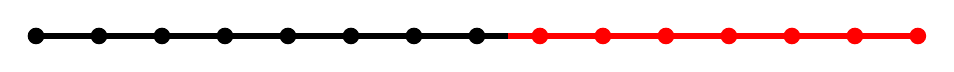
\begin{tikzpicture}
\def\n{13}\def\s{0.8}
\pgfmathsetmacro{\xr}{14*\s}
\pgfmathsetmacro{\xmid}{(7*\s + 8*\s)/2}
\draw[line width=2pt, black] (0,0) -- (\xmid,0);
\draw[line width=2pt, red] (\xmid,0) -- (\xr,0);
\fill[black] (0,0) circle (3pt);
\foreach \i in {1,...,13} {
    \ifnum\i>7
        \fill[red] (\i*\s,0) circle (3pt);
    \else
        \fill[black] (\i*\s,0) circle (3pt);
    \fi
}
\fill[red] (\xr,0) circle (3pt);
\end{tikzpicture}
\vspace{0.5em}
\caption{Schematic depicting the how the suction extents are varied while maintaining a constant suction coefficient over this region. Transition is expected to occur at the rightmost node and the red nodes represent the suction extent for 7 of the 15 nodes.}
\label{fig:suction-extent}
\end{figure}

\begin{table}[!t]
\centering
\caption{Summary of results for infinite swept wing while varying the suction extent upstream of the transition location and maintaining a constant suction coefficient.}
\label{tab:suction-extent}
\begin{tabular}{ccc}
\toprule
Configuration & $v_{\text{suc}}$ & $C_D$ (counts) \\
\midrule 
Baseline  & - & 60.25 \\
\midrule
\textbf{Suction Nodes} & & \\
15/15 Nodes & $0.0100 \: U_\infty$ & 58.67 (-2.62\%)  \\
14/15 Nodes & $0.0107 \: U_\infty$ & 58.70 (-2.57\%)  \\
13/15 Nodes & $0.0115 \: U_\infty$ & 58.73 (-2.52\%)  \\
12/15 Nodes & $0.0125 \: U_\infty$ & 58.75 (-2.49\%) \\
11/15 Nodes & $0.0136 \: U_\infty$ & 58.79 (-2.42\%)  \\
10/15 Nodes & $0.0150 \: U_\infty$ & 58.83 (-2.36\%)  \\
9/15 Nodes & $0.0167 \: U_\infty$  & 58.87 (-2.29\%)  \\
8/15 Nodes & $0.0188 \: U_\infty$  & 58.95 (-2.16\%)  \\
\bottomrule
\end{tabular}
\end{table}

\clearpage

\subsubsection{Wall Porosity Considerations}
This section investigates wall porosity considerations using a coefficient to allocate part of the drag over the specified region as suction drag and the rest as skin friction and pressure drag, treating it as a solid wall. This results in the overall drag over the suction region being defined as:

\begin{equation}
C_{\text{d,total}} = (1-p) \cdot (C_{\text{d,f}} + C_{\text{d,p}}) + p \cdot C_{\text{d,suc}},
\label{eq:porosity}
\end{equation}

\noindent where $p$ is the porosity of the region and $C_{\text{d,suc}}$ is the suction drag defined in Equation \ref{eq:suction-drag}. The results for the application of suction in Table \ref{tab:wall-porosity-results} demonstrate that when suction is applied from 20\% -- 25\% chord on the upper surface, there is small change overall drag coefficient. The small variation in overall drag with porosity is expected, as the suction extent is small and located in an area where the boundary layer is already relatively thin. As a result, the contribution of suction drag to the total drag is modest, and the redistribution between suction and skin-friction drag has limited influence. For configurations where suction is distributed over a larger chordwise extent, the suction drag contribution would represent a larger proportion of the total drag.

\begin{table}[!t]
\centering
\caption{Summary of results for infinite swept wing while varying the porosity of the surface over which suction is applied. A suction coefficient of $\mathbf{C_Q = 0.0001}$ is used.}
\label{tab:wall-porosity-results}
\begin{tabular}{cccc}
\toprule
Porosity & $C_{\text{d,total}}$ (counts) & L/D \\
\midrule
1.00 & 58.67 & 79.03 \\
0.10 & 58.95 (0.47\%) & 78.65 \\
0.20 & 58.92 (0.43\%) & 78.69 \\
0.30 & 58.89 (0.37\%) & 78.74 \\
0.40 & 58.86 (0.33\%) & 78.78 \\
0.50 & 58.83 (0.27\%) & 78.82 \\
\bottomrule
\end{tabular}
\end{table}

\section{Conclusions}
\label{sec:conclusion}
In this paper, we present a framework for aerodynamic shape optimization incorporating Hybrid Laminar Flow Control (HLFC) through active boundary-layer suction. The methodology was first validated against benchmark cases including flat-plate flow and NACA 64A010 airfoil experiments, demonstrating accurate prediction of laminar-to-turbulent transition and suction effects. Lift-constrained drag minimization was then performed for airfoils and infinite swept wings with fixed suction applications. For infinite swept wings at Airbus A340 and A350 operating conditions, aerodynamic shaping combined with suction delayed crossflow-dominated transition, yielding substantial drag reductions beyond those achieved by geometry-only NLF optimization. The results also highlighted diminishing returns at higher suction levels and demonstrated that moderate suction can deliver significant performance gains while keeping suction drag and pump-power penalties low.

Future work will focus on extending this framework to three-dimensional, finite wings to capture realistic planform effects and full spanwise flow behavior. Optimization of suction power and placement will also be incorporated to identify the most effective combination of suction intensity and location for drag reduction while minimizing energy expenditure. These developments will enable more realistic assessments of HLFC performance for practical aircraft configurations and support the design of efficient suction-based laminar flow control systems.



\section*{Acknowledgements}
This work is partially funded by Bombardier, Transport Canada, the Natural Sciences and Engineering Research Council (NSERC), and the University of Toronto. All results in this paper were computed on the Niagara and Trillium supercomputers at the SciNet HPC Consortium, a part of the Digital Research Alliance of Canada.

\pagebreak 

\bibliography{MyLibrary}

\end{document}